\documentclass{article}
\usepackage[francais]{babel}
\def\printlandscape{\special{landscape}} % Works with dvips.
\usepackage{geometry}
\geometry{ hmargin=3cm, vmargin=2.5cm } % set margin
\usepackage{graphicx}% include image
%\usepackage{pstricks,pst-node,pst-tree}
%\usepackage{amssymb}
\usepackage[utf8]{inputenc}
\usepackage[T1]{fontenc}
\usepackage{fancybox} % for shadow and Bitemize
\usepackage{alltt}
\usepackage{graphicx}
%\usepackage{epsfig}
%\usepackage{fullpage}
%\usepackage{fancyhdr}
%\usepackage{moreverb}
%\usepackage{xspace}
\usepackage[colorlinks,hyperindex,bookmarks,linkcolor=blue,citecolor=blue,urlcolor=blue]{hyperref}
\usepackage{placeins}
\usepackage{wrapfig}
\usepackage{epsf}
\setcounter{secnumdepth}{4}
\setcounter{tocdepth}{3}
\makeatletter
\newcounter {subsubsubsection}[subsubsection]
\renewcommand\thesubsubsubsection{\thesubsubsection .\@alph\c@subsubsubsection}
\newcommand\subsubsubsection{\@startsection{subsubsubsection}{4}{\z@}%
                                     {-3.25ex\@plus -1ex \@minus -.2ex}%
                                     {1.5ex \@plus .2ex}%
                                     {\normalfont\normalsize\bfseries}}
\newcommand*\l@subsubsubsection{\@dottedtocline{3}{10.0em}{4.1em}}
\newcommand*{\subsubsubsectionmark}[1]{}
\makeatother


\title{Analyse Syntaxique}
\author{Mohammed Akram Rhafrane - Ismail Senhaji - Nathanael Bertrand - Mehdi Boutchiche\\}
\date{\today} 
\begin{document}




\begin{figure}[t]
	\centering
		
\includegraphics[width=0.60\textwidth]{logo-ups.jpg}
	\label{fig:logo-ups}
\end{figure}
\newline
\maketitle

\newpage
\tableofcontents

\newpage
\begin{abstract}
Résumé du contenu du document.
\end{abstract}

%-----------------------------------------------------------
\newpage
\section{Introduction}
\label{hints}

\newpage
\section{Fondamenteux}
\label{hints}
\subsection{Langages et grammaires}
\subsubsection{Défintion}
Un langage formel est un ensemble de mots constitués de symboles qui appartiennent à son alphabet.
Un langage formel est décrit par une grammaire.
De manière générale, une grammaire est définie par un quadruplet:

    N : l’ensemble des non-terminaux utilisés pour décrire les règles de productions

    X : l’ensemble des terminaux, c’est à dire les symboles ou encore l’alphabet

    P : l’ensemble des règles de production

    S : l’axiome, c’est un élément de N
\newline

Ainsi, la notation: G(L) = <N, X, P, S> décrit la grammaire G associée au langage L.
Les grammaires sont analysées par des automates. Il existe plusieurs types d’analyses de grammaires qui font appels à plusieurs types d’automates.
Dans le monde de la compilation l’analyseur syntaxique fait référence à l’algorithme qui met en oeuvre l’automate d’analyse d’une grammaire.
Dans cet écrit, nous nous attarderons sur deux types d’analyseurs: les analyseurs de type LL et ceux de type L(AL)R.

\subsubsection{Grammaires ambiguë}
On dit qu’une grammaire est ambiguë  lorsqu’on peut trouver deux arbres de dérivation différents pour le même mot.
Les grammaires ambiguë pose un problème lors de la compilation, c’est pour ça qu’il est préférable de les transformer en grammaire non ambiguë si c’est possible.\newline
\textit{Exemple : }\newline\newline
Prenons la grammaire suivante G=( \textit{\{E\} , \{a,+,}x\textit{\} , R , E} ) \newline
Avec \textit{R} donné par : \textit{E := E} x \textit{E | E + E | a}


\begin{figure}[h!]
	\centering
		
\includegraphics[width=0.90\textwidth]{grammaireAmbigue.png}
	\label{fig:grammaireAmbigue}
\end{figure}\FloatBarrier

Donc nous remarquons qu'on peut construire deux arbres de dérivation à partir de la chaîne de caractères 
\textit{"a + a} x \textit{a"} 

\subsection{Analyse lexicale}
l’analyse lexicale consiste à découper une chaîne de caractère en unités lexicales ou lexèmes à la demande de l’analyseur lexicale.
Il est définit par un ensembles d’expressions relationnelles qui exigent certaines séquences de caractère pour former les lexèmes.
\textit{Exemple :}

\begin{figure}[h!]
	\centering
		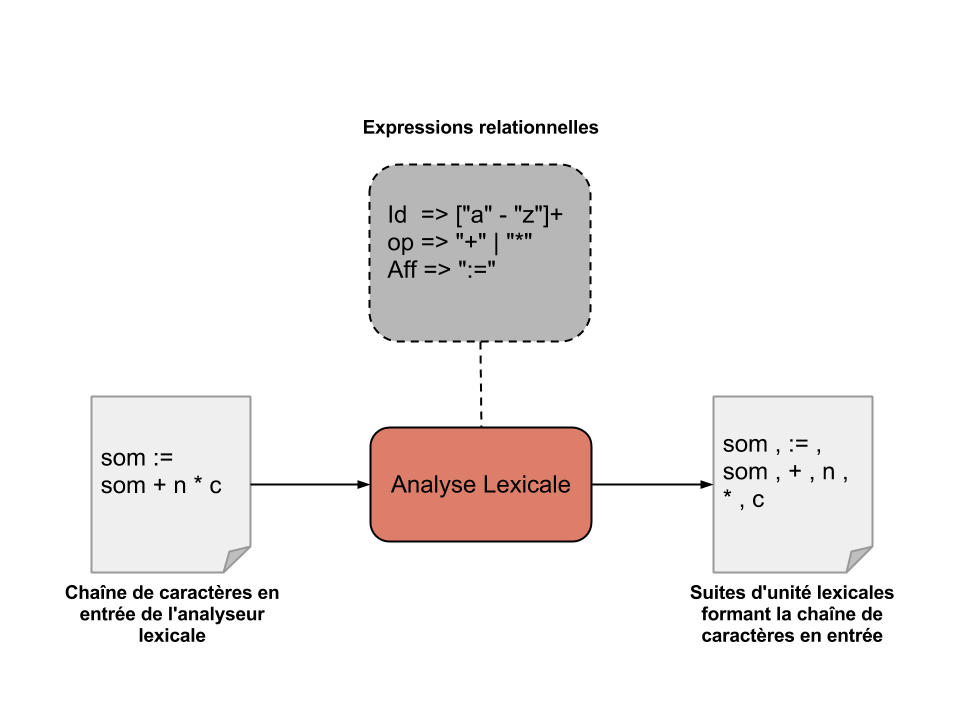
\includegraphics[width=0.80\textwidth]{AnalyseLexicale.png}
	\caption{Analyse lexicale}
	\label{fig:AnalyseLexicale}
\end{figure}\FloatBarrier


\subsubsection{Unités lexicales}
Une unité lexicale ou un lexème est une chaîne de caractère qui correspond à un symbole. à l’aide du processus de segmentation, on peut extraire à partir d’un flux de caractères entrant une suite d’unités lexicales, ensuite c’est l’analyseur lexicale qui traitent ces lexème et les rangent dans des catégories d’entités lexicales.

\subsubsection{Analyseur Lexicale}

On appelle analyseur lexical \cite{refAnalyseurLexicale}, lexeur, ou encore scanneur, tout programme effectuant une analyse lexicale. Il s'agit le plus souvent d'une unique fonction qui sera appelée par l'analyseur syntaxique (voir Analyse syntaxique) ou par une autre fonction.

Le scanneur contient toutes les informations sur les séquences de caractères qui peuvent être contenues dans les entités lexicales qu'il génère. Par exemple, une entité lexicale de type « INTEGER » peut contenir n'importe quelle séquence de caractères numériques (chiffres).
\begin{itemize}
\item Son rôle consiste à :
			\item Eliminer les « bruits » du texte source : commentaires, espaces, …
			\item Reconnaître les opérateurs et les mots-clés : ==, if, …
			\item Reconnaître les chaînes de caractères, les identificateurs et les constantes numériques
\end{itemize}
Il produit en sortie une entité lexicale qui sera utilisée par l'analyseur syntaxique.
\begin{itemize}
\item Un analyseur lexical peut être écrit :
			\item « à la main » : il faut construire l'automate fini non déterministe à partir d'une expression rationnelle E, puis l'exécuter pour déterminer si une chaîne d'entrée appartient au langage reconnu par E
			\item Par une table décrivant l'automate et un programme exploitant cette table
			\item Par un générateur d'analyseurs : Flex, ANTLR, Lex, etc.
\end{itemize}    

\subsubsection{Segmentation}
La segmentation est le fait de séparer les différentes sections d’une chaînes de caractères, par exemple pour une phrase l’ordinateur la considère comme une chaîne de caractère et non pas une suite de mot, le rôle de la segmentation est donc de faire une séparation entre ces mots selon le caractère de séparation dans ce cas le caractère espace.

\subsection{Analyse syntaxique}
Le rôle de l’analyse syntaxique \cite{refAnalyseSyntaxique} est de savoir si une phrase appartient à la syntaxe d’un langage.
A partir du flot de lexèmes construits par l’analyse lexicale dans un premier temps, l’analyse syntaxique permet de générer un arbre de syntaxe abstraite.
Cet arbre est construit à base d’un ensembles de règles définissant une grammaire formelle sur laquelle est basé le langage en question.
l’analyse syntaxique permet plus particulièrement de détecter les erreurs de syntaxe en continuant tout de même l’analyse pour éviter les cycles de compilation/correction pour les développeurs.\newline
\textit{Exemple :}\newline
Reprenant l'exemple de d'analyse lexicale \ref{fig:AnalyseLexicale}. L'analyse lexicale a construit une suites d'unités lexicales a partir d'une chaîne de caractères en entrée.\newline
Maintenant le rôle de l'analyse syntaxique est de reprendre ce résultat et essayer de construire un arbre de syntaxe suivant la grammaire qui définit le langage afin de s'assurer que la chaîne de caractères appartient au langage.

\begin{figure}[h!]
	\centering
		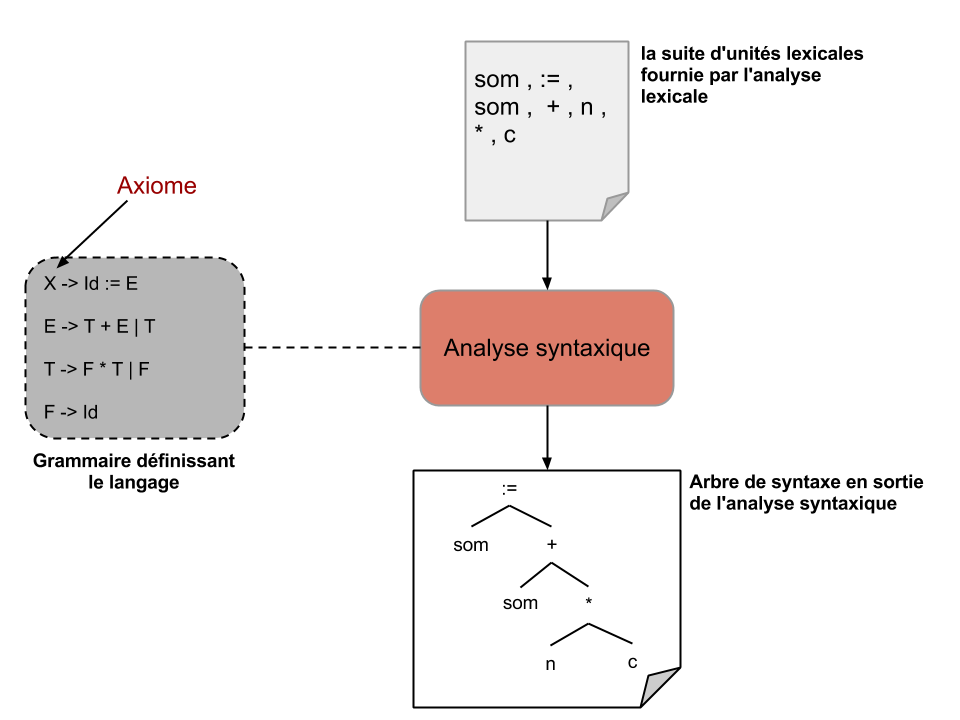
\includegraphics[width=0.80\textwidth]{AnalyseSyntaxique.png}
	\caption{Analyse syntaxique}
	\label{fig:AnalyseSyntaxique}
\end{figure}\FloatBarrier


\subsubsection{Analyseur syntaxique}

L'analyseur syntaxique est une programme qui reçoit une suite d'unités lexicales de la part de l'analyseur lexicale et doit vérifier que cette suite est engendrée par la grammaire du langage décrit.

Voici un schema montrant les intéractions entre l'analyseur lexicale et l'analyseur syntaxique:

\begin{figure}[h!]
	\centering
		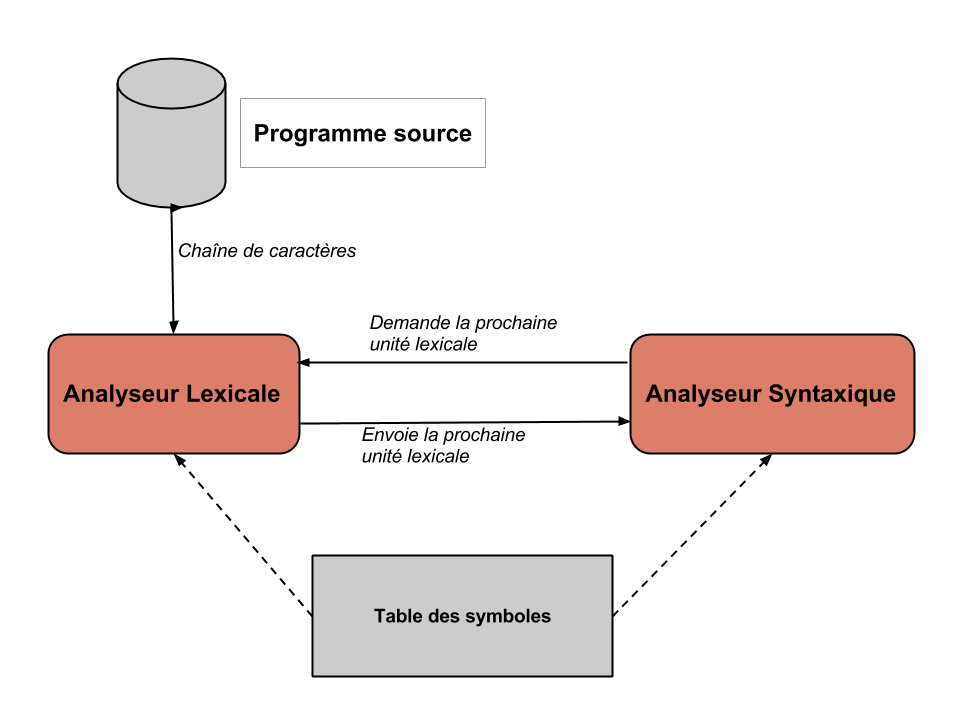
\includegraphics[width=0.70\textwidth]{interactionLexSynt.png}
	\caption{Interaction entre l'analyseur lexicale et l'analyseur syntaxique}
	\label{fig:interactionLexSynt}
\end{figure}\FloatBarrier
\newline
un analyseur syntaxique doit retracer le cheminement d’application des règles qui ont menées à l’axiome. Pour ça, il existe deux types d’analyse:

\subsubsection{Analyse descendante}\label{sec:analyseDes}
Le principe de l’analyse descendante est de partir de l’axiome en suivant les règles de production afin de retrouver le texte analysé. Ce type d’analyse procède en découpant le texte petit à petit jusqu'à retrouver les unité lexicale. L’analyse LL est un exemple d’analyse descendante.\newline
\textit{Exemple :}\newline
On a :\newline
S => aSbT | cT | d\newline
T => aT | bS | c \newline
et la chaîne suivante en entrée W=acbbadbc\newline
On part avec l'arbre contenant le seul sommet S.
La lecture de la première lettre du mot (a) nous permet d'avancer la construction de l'arbre avec :

\begin{figure}[h!]
	\centering
		
\includegraphics[width=0.70\textwidth]{AnalyseDescendante1.png}
	\label{fig:AnalyseDescendante1}
\end{figure}\FloatBarrier

Puis la deuxième lettre nous amène à :

\begin{figure}[h!]
	\centering
		
\includegraphics[width=0.70\textwidth]{AnalyseDescendante2.png}
	\label{fig:AnalyseDescendante2}
\end{figure}\FloatBarrier

et ainsi de suite jusqu'a la fin du mot.

\begin{figure}[h!]
	\centering
		
\includegraphics[width=0.70\textwidth]{AnalyseDescendante3.png}
	\label{fig:AnalyseDescendante3}
\end{figure}\FloatBarrier

Donc le mot appartient au langage. Sur cet exemple c'est simple car chaque règle commence par un terminal différent ce qui facilite le choix de la règle à appliquer. Mais c'est pas toujours le cas, dans la plus part des cas on se trouve devant le choix entre plusieur règles par exemple si on considère :\newline
S => aAb\newline
A => cd | c \newline
et on veut lire le mot W=acb\newline
On se retrouve avec

\begin{figure}[h!]
	\centering
		
\includegraphics[width=0.70\textwidth]{AnalyseDescendante4.png}
	\label{fig:AnalyseDescendante4}
\end{figure}\FloatBarrier

En lisant le caractère "c", on ne sait pas si il faut choisir la règle A => cd ou bien A => c.
Pour le savoir il faut lire le caractère suivant "b", ou alors, il faut se donner la possibilité de de faire des retours en arrière :
On essaye la première règle, on aboutit à un echec, alors on retourneen arrière pour essayer la deuxième règle.

\subsubsection{Analyse ascendante}
L’analyse ascendante d’une autre part, procède contrairement à l’analyse descendante en retrouvant le cheminement à partir du texte analysé. Ce type d’analyse essaye de regrouper les unité lexicale entre elles pour retrouver l’axiome. L’analyse LR est un exemple d’analyse ascendante.
Reprenons l'exemple dernier \ref{sec:analyseDes} :
Cette fois en utilisant une analyse ascendante, on va partir de la chaîne de caractères pour retrouver l'axiome S.
La chaîne analysé est la même du dernier exemple \newline W=accbbadbc\newline\newline\newline
\begin{tabular}{|E|D|}
\hline
\textbf{a}ccbbadbc & Aucune règle à appliquer\\
\hline
a\textbf{c}cbbadbc & Aucune règle à appliquer\\
\hline
ac\textbf{c}bbadbc & T => c\\
\hline
ac\textbf{T}bbadbc & S => cT\\
\hline
a\textbf{S}bbadbc & Aucune règle à appliquer\\
\hline
aS\textbf{b}badbc & Aucune règle à appliquer\\
\hline
aSb\textbf{b}adbc & Aucune règle à appliquer\\
\hline
aSbb\textbf{a}dbc & Aucune règle à appliquer\\
\hline
aSbba\textbf{d}bc & S => d\\
\hline
aSbba\textbf{S}bc & Aucune règle à appliquer\\
\hline
aSbbaS\textbf{b}c & Aucune règle à appliquer\\
\hline
aSbbaSb\textbf{c} & T => c\\
\hline
aSbbaSb\textbf{T} & S => aSbT\\
\hline
aSbb\textbf{S} & T => bS\\
\hline
aSb\textbf{T} & S => aSbT\\
\hline
S & Axiome retrouvé\\
\hline
\end{tabular}
\newline\newline\newline
Alors le mot "accbbadbc" est bien dans le langage.

\subsubsection{Analyse deterministe}

Un analyseur syntaxique, en tant que système de réécriture, est déterministe si une seule règle de réécriture est applicable dans chaque configuration de l'analyseur. Par extension, il ne peut alors y avoir qu'une seule séquence de règles permettant d'analyser le texte dans sa totalité, et donc celui-ci ne peut être syntaxiquement ambigu. Toutefois, il peut être fait usage de techniques telles que la pré-vision (en anglais lookahead) ou le backtracking pour déterminer quelle règle il faut appliquer à un point donné de l'analyse.

Les méthodes d'analyse déterministes sont principalement employées pour l'analyse des langages de programmation. Par exemple, les analyses LR, LL, ou LALR (employée par Yacc) sont toutes déterministes. On ne peut cependant pas construire un analyseur déterministe pour n'importe quelle grammaire non contextuelle. Dans ce cas, et si l'on souhaite n'avoir qu'une seule analyse en sortie, on est contraint de lui adjoindre des mécanismes supplémentaires, comme des règles de désambiguïsation ou des modèles probabilistes permettant de choisir la « meilleure » analyse.

Une méthode d’analyse descendante et déterministe est dite prédictive \cite{refAnalyseSyntaxique}.

\subsubsection{Analyse non deterministe}

La taille et la complexité des langues naturelles, sans oublier leur inévitable ambiguïté, rend leur analyse déterministe totalement impossible. Une analyse non déterministe s'apparente à une résolution dans un système contraint, et s'exprime assez aisément en Prolog.

L'emploi de méthodes tabulaires, mémorisant les calculs intermédiaires, sera plus efficace qu'un simple backtracking. L'analyse CYK est un exemple d'analyse tabulée, à laquelle on préférera des méthodes plus sophistiquées

    d'analyse à chartes comme l'analyse Earley
    ou d'analyse LR généralisée (GLR).

Ces deux dernières méthodes d'analyse sont aussi appréciées pour l'analyse de langages de programmation dont la syntaxe est ambiguë, comme par exemple C++.

\subsubsection{Récupération des erreurs}

En analyse syntaxique des langages de programmation, il faut être capable de continuer l'analyse même lorsque le code source contient des erreurs, pour éviter des cycles de compilation/correction fastidieux pour le développeur. De même, en analyse syntaxique des langues naturelles, il faut pouvoir analyser des énoncés même s'ils ne sont pas couverts par la grammaire, inévitablement incomplète. La récupération sur erreur, ou rattrapage d'erreur (anglais error recovery), doit être suffisamment efficace pour détecter les problèmes, et "faire avec", moyennant une correction du source ou la faculté de produire des analyses (légèrement) déviantes par rapport à la grammaire. On peut citer quelques approches qui vont dans ce sens.

\subsubsubsection{Mode panique}

le mode panique \cite{refModePanique} est un cas particulier de mode dégradé, c’est-à-dire une méthode de récupération sur erreur.
Par exemple, lorsqu'une erreur survient lors d'une analyse syntaxique, l'analyseur supprime un à un chaque prochain symbole jusqu'à ce qu'il atteigne un symbole permettant de se resynchroniser.

\subsubsubsection{Production erreurs}

L'utilisation de productions erreurs \cite{refProductionErreurs} est une méthode de récupération sur erreur. Elle consiste à ajouter à la grammaire d'un langage des productions contenant la notion d'erreur. Cette technique est notamment utilisée par Yacc.

\subsubsubsection{Correction locale}

La correction locale \cite{refCorrectionLocale} est une technique de récupération sur erreur. Lorsqu'un analyseur constate une erreur lors de la lecture d'un symbole, il remplace le symbole lu par un autre qui lui semble plus juste.


\subsection{LL(*)}
Descente récursive ou prédicative: pour les grammaires simple ou le premier symbole terminal fournie des informations suffisantes pour choisir la règle de production.
Pas possible si grammaire récursive à gauche.
Besoin de factorisation à gauche lorsque 2 règles commencent par le même lexème.
Mais cette méthode à une faiblesse, c’est qu’elle doit toujours prédire qu’elle règle utiliser \cite{refModernCompiler}.

\subsection{L(AL)R}
Dérivation à droite permet de rapporter le choix de la règle de production à utiliser.
Elle commence du bas vers le haut.
L’algorithme s’arrête quand tous les caractères ont été lus. La chaîne est accépté si la partie analysée se réduit à l’axiome 
\cite{refModernCompiler}.

\section{Comparaison entre les outils}
\label{hints}

\subsection{Yac/Bison/Cup}


\subsubsection{Yac - Yet Another Compiler-Compiler}
YACC est un programme qui permet de générer un analyseur syntaxique à partir d’une spécification. La spécification est l’ensemble des règles de grammaire associées au langage à analyser.
L’analyseur ainsi généré est de type LALR(1).

\subsubsection{Specification}
La spécification est l’ensemble des données qui permettront à YACC de générer l’analyseur. Elle décrit le langage qui sera reconnu sous forme de règles de grammaires. De cette façon l’analyseur a les connaissances pour définir si un flux donné en entrée est syntaxiquement correcte par rapport à sa spécification.
Cependant, un analyseur syntaxique est souvent utilisé dans le contexte de traduction de langage. La spécification permet cette fonctionnalité puisqu’il est possible de spécifier des actions associées aux règles de grammaire.

La spécification suit la structure suivante :

Bloc des déclarations

%%

Règles de grammaire

%%

Programme

Les sections “Bloc des déclarations” et “Programme” sont facultatives.

Une règle de grammaire est notée sous la forme:

A : B { /* action pour cette regle */ };

Ci-dessous un exemple de spécification Yacc qui génère une calculatrice très minimaliste.

Ici, on utilise Yacc sans Lex afin de comprendre le fonctionnement. Cependant, il faut définir à la main la fonction yylex(). Celle-ci renvoie un entier qui indique le type de token qui a été reconnu en entrée.

%{
    \#include <ctype.h>
    \#include <stdio.h>
    \#include <stdlib.h>
%}

%token CHIFFRE

%%
ligne : commande '\\n' ligne
    | '\\n' \{ printf("Fin du programme\\n"); exit(0); \}
    ;

commande: expr \{ printf("Resultat: \%d\\n", \$1); \};


expr : expr '+' terme \{ \$\$ = \$1 + \$3; \}
    | terme
    ;
   
terme : terme '*' facteur \{ \$\$ = \$1 * \$3; \}
    | facteur
    ;
   
facteur : '(' expr ')' \{ \$\$ = \$2; \}
    | CHIFFRE
    ;

%%
int main()\{
    yyparse();   
\}

int yyerror(char *s)\{
    printf("\%s \\n", s);
\}


int yylex()\\{
    int c;
    c = getchar();
    if(isdigit(c))\{
        yylval = c-'0';
        return CHIFFRE;
    \}
    return c;
\}

Pour faire fonctionner cet exemple, il faudra entrer les lignes de commande suivantes:

> bison exemple1.y

> gcc exemple1.tab.c -o exemple1

> ./exemple1

Dans cet exemple, on a défini 5 règles. À quelques unes de ces règles on a associé des actions afin d’effectuer les calculs sur les chiffres lus.

Ces actions sont des instructions C dans lesquelles on a accès à des variables spéciables.
Ainsi les variables \$n font référence à la valeur du n-ième élément de droite et \$\$ fait référence à l’élément de gauche.

\subsection{ANTLR}
Pour obtenir une certaines flexibilité et une meilleures gestion d’erreurs, les programmeurs préfèrent écrire leurs parseurs de descente récursive à la main, nous allons donc vous présentez dans ce chapitre un outil, qui combine flexibilité, gestion d’erreurs  et présente tout les avantages d’un générateur de parseur, c’est outil est ANTLR.
\subsubsection{Défintions}
ANTLR \cite{refANTLR} est un générateur de parseur public, il propose plusieurs fonctionnalités qui rendent sont utilisation simple, il propose  des prédicats qui permettent aux programmeurs de diriger et de contrôler e le parseur grâce à des expressions syntaxique et sémantique.
ANTLR permet aussi d’intégrer des  descriptions lexicales et syntaxiques  et peut générer automatiquement l’arbre syntaxique.
\subsubsection{Fonctionnement}
Comme ce qui a été dit précédemment dans l’introduction, les prédicats permettent de diriger le parseur, ainsi ANTLR peut générer des parseurs pour plusieurs et différents langages.
Les prédicats sémantiques indiquent la validité sémantique d’une production, les prédicats syntaxiques sont quant à eux des fragments de grammaires qui décrivent un contexte syntaxique qui doit être satisfait avant de reconnaître une production associé.
\subsubsection{Fonctionnalités}
Fort d’une stratégie puissante autant que parseur, ANTLR a plusieurs fonctionnalités qui rendent sont utilisation plus agréables que d’autres LR/LALR et LL générateurs de parseurs.
\begin{itemize}
\item ANTLR  intègre la spécification entre une analyse lexicale et syntaxique.
			\item ANTLR facilite la construction de l’arbre syntaxique.
			\item ANTLR génère des parseurs de descente récursives en C et C++.
			\item ANTLR   facilite la gestion d’erreurs.
			\item ...
\end{itemize}
\subsubsection{Diagramme de flux}


\subsubsection{Eléments de langages}
Le tableau illustre quelques éléments de langage spécifique à ANTLR qui le distinguent des autres générateurs de parseurs.
\newline

\begin{tabular}{|E|D|X|}
\hline
Elément de langages & Description & Exemple \\
\hline
Token & Commence par majuscule & ID \\
\hline
\prec\prec...\succ\succ & Définie une action sémantique & \prec\prec printf\left("\%S",a\right);\succ\succ \\
\hline	
\left(...\right) & Régle & \left("int" \left| ID \right| storage\_class\right) \\
\hline
\left(...\right)* & Closure & ID\left("\," ID\right)* \\
\hline
\left(...\right)+ & Positive Closure & slist : \left( stat | SEMICOLON \right) \+ \; \\
\hline
\left\{...\right\} & Optionnel & \left\{ELSE stat\right\} \\
\hline
\prec\prec...\succ\succ? & Prédicat sémantique & type : \prec\prec is\_Type\left(str\right)\succ\succ ? ID \; \\
\hline
\left(...\right)? & Prédicat syntaxique & \left(\left(list EQ\right)\right)? list EQ list | list \right) \\
\hline
\end{tabular}
\subsubsection{Langage et description}
\subsubsubsection{Description de langage et ANTLR}
Une description ANTLR est un collection de règles et d'actions précéder par une en-tête dans laquelle l'utilisateur définies les types des attributs par exemple.\newline Une règles ANTLR est entre autre une liste d'alternative séparer par"|":\newline
règle : \textit{alternative \textsl{1}} | \textit{alternative \textsl{2}} |... |\textit{alternative \textsl{n}};\newline
Chaque alternative est composée d'une liste d'éléments.Les règles définissent aussi des arguments et retournent des valeurs, dans l'exemple suivant, il y a \textsl{n} arguments et \textsl{m} valeurs retournées:\newline
\textit{règles}[\textit{args \textsl{1}},...,\textit{args \textsl{n}}] > [\textit{returnVal \textsl{1}},...,\textit{returnVal \textsl{m}}]\newline
Notons aussi qu'une description ANTLR est diffèrents de celle des autres parseurs générateurs car les expressions régulières sont spécifiées (\#token ID) ou directement référencées (\#segment). Ces spécifications lexical ou grammatical se trouvent dans un fichier, ainsi plus besoin de mantenir deux spécifications. ANTLR assigne automatiquement le type des unités lexicales et génère l'analyseur syntaxique.
Autre point important, ANTLR optimise le choix du nombre de lookahead en utilisant le moins possible. En effet, ANTLR génère une décision qui utilise un symbole qui distingue entre la première alternative et les autres. Ainsi, le prgrammeur utilise la puissance d'un parseur LL(k) avec k > 1 sans se soucié de l'efficacité ou non du parseur. Par exemple, si une règle requiert trois symboles pour différencier entre deux alternatives, ANTLR s'en occupe et génère un symbole pour faire la différence.
ANTLR permet aussi à l'utilisateur de définir des actions et de les appelées là où il veut dans une production ANTLR, ces actions sont utilisées pour améliorer les tests sémantiques, générer une représenation intermédiaire ou directement générer la traduction.
\subsubsubsection{Prédicats}
ANTLR supporte l'utilisation de prédicats sémantique et syntaxique qui permet à l'utilisateur d'indiquer la validté sémantique et syntaxique d'une production, permettant ainsi à ANTLR de gérer naturellement des situations d'analyse difficile.
\subsubsection{Quelques fonctionnalités utile aux programmeurs}
\subsubsubsection{Intégration de l'analyse syntaxique et lexicale}
Une description ANTLR contient à la fois une spécification pour l'analyse des unités lexicale et la spécification du parseur lui-même, ce qui élimine le besoin d'avoir deux fichiers différents pour chaque spécification, en effet ANTLR extrait automatiquement une description de l'analyseur lexicale à partir de la description intégrée de ANTLR.
ANTLR permet ainsi l'utilisation de plusieurs analyseurs lexicaux dans la même description ANTLR, cette pratique permet alors l'analyse de plusieurs langages.
\subsubsubsection{Gestion d'erreurs}
ANTLR propose deux mécanismes pour la gestion des erreurs.Dans le premier mécanisme, ANTLR génère un message d'erreur en utilisant une simple heuristique qui est suffisante pour plusieurs applications. par contre, quand une gestion d'erreurs plus complexe est requise, ANTLR fourni un second mécanisme appeler Parseur de gestion d'Exception qui offre une construction de rapport plus flexible dans un framework convenant.
Le premier mécanisme génère automatiquement des rapports d'erreurs, désigne là où l'erreur à été détecter et qu'est ce qui était attendu.
Le premier mécanisme, qui génère automatiquement des rapports d'erreurs, désigne là l'erreur à été détecter et qu'est ce qui était attendu.
Le second mécanisme quant à lui, fournis un framework pour y mettre les rapports d'erreurs sémantiques et syntaxiques, notons que le premier mécanisme ne reconnait pas les erreurs sémantiques.
\subsubsubsection{Construction de l'arbre syntaxique}
Le plus souvent, les parseurs construisent une forme intermédiaire qui sera utilisé plus tard dans des phases de compilation par exemple. En utilisant quelques annotations, ANTLR peut automatiquement construire un arbre syntaxique, évitant ainsi à l'utilisateur d'appeler la construction d'un arbre à chaque fois.
Pour créer un arbre, l'utilisateur des annotations grammaticales qui indiquent le noeud père, les feuilles et aussi qui doit être exclu de l'abre. Les unités lexicales précédés de "!" par exemple, son à exclure de l'arbre.Toutes les autres unités lexicales sont considérées comme des feuilles.
\subsection{Xtext}
\subsubsection{Definition}
Xtext est un framework pour le développement de langages de programmation et de DSL(Domain Specific programming language).
Le framework Xtext s’appuie sur sur une grammaire générée ANTLR ainsi que le framework de modelisation EMF.

Il fonctionne sur une JVM (Machine Virtuelle Java) et est constitué de plusieurs API qui vous permettent de décrire les différents aspects du langage que vous voulez créer et propose une implémentation complète de ce langage. Notons que le langage développé sera alors un langage qui s'appuie et qui surcouche le langage Java. C'est-à-dire que les objets offerts par ce framework sont complètement des objets Java et le développement du compilateur de votre langage sera alors écrit en Java.

Xtext peut servir entre autres à proposer des solutions dans les domaines tels que : les systèmes embarqués, l'automobile, les appareils mobiles, l'automatique, les jeux vidéo, etc.

Notons aussi que les langages développés via Xtext peuvent selon son tutoriel être définis non seulement avec le langage Java, mais aussi d'autres langages tels que C, C++, C# objective C, Python et Ruby. De plus, une fois que le DSL est mis en œuvre , son utilisation devient indépendante de la JVM. 

Xtext couvre tous les aspects d’un IDE moderne : parseur, compilateur ,interpreteur et integration complete dans l’environnement de developpement Eclipse.

Xtext fournit un environnement convivial aux utilisateurs d’un DSL.

\subsubsection{Definition DSL}
DSL:est un langage de programmation dont les spécifications sont à un domaine d’applications précis , la construction des langages dédiés diffère fondamentalement de celle d’un langage classique, le processus de développement  peut s'avérer très complexe, sa conception nécessite une double compétence sur le domaine à traiter et en développement informatique(exp :SQL:destiné à interroger ou manipuler une base de données relationnelle)

\subsubsection{Definition Eclipse}
Eclipse IDE est un environnement de développement intégré libre (le terme Eclipse désigne également le projet correspondant, lancé par IBM) extensible, universel et polyvalent, permettant potentiellement de créer des projets de développement mettant en œuvre n'importe quel langage de programmation. Eclipse IDE est principalement écrit en Java (à l'aide de la bibliothèque graphique SWT, d'IBM), et ce langage, grâce à des bibliothèques spécifiques, est également utilisé pour écrire des extensions.

La spécificité d'Eclipse IDE vient du fait de son architecture totalement développée autour de la notion de plug-in.


\subsubsection{Fonctionnalités Xtext}
Parmi les fonctionnalités qu’offre Xtext:
\begin{itemize}
			\item -coloration syntaxique: Suivant les éléments de la grammaire , Xtext propose une coloration syntaxique entièrement     personnalisable.
			\item -auto complétion: auto complétion sur les éléments du langage 
			\item -validation: Xtext valide le contenu de l'éditeur à la volée, produisant ainsi un retour direct à l’utilisateur en cas d’erreur de syntaxe.
			\item -intégration avec d’autres composants Eclipse 
\end{itemize}

\subsubsection{Diagramme de flux}



\begin{figure}[h]
	\centering
		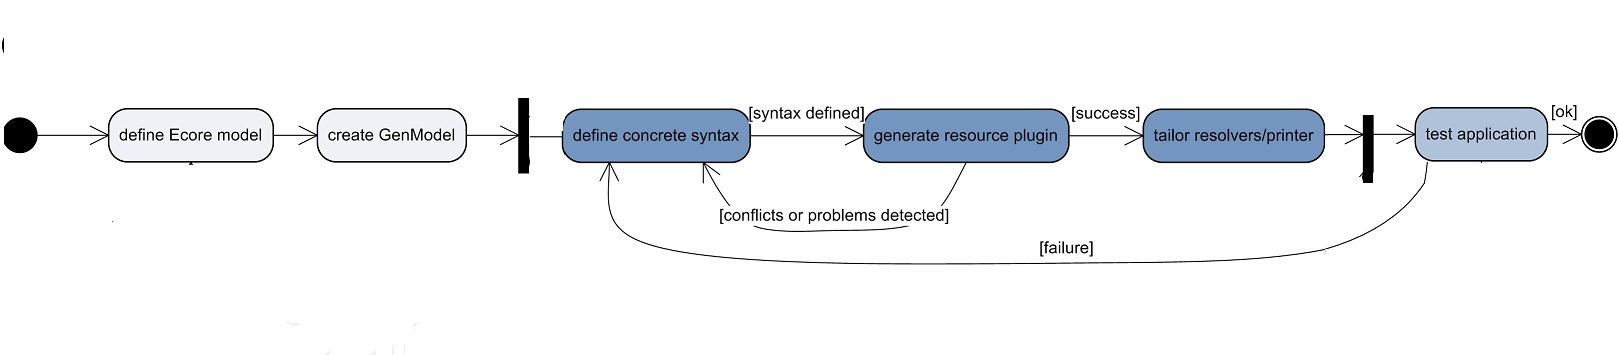
\includegraphics[width=0.80\textwidth]{Emftext_process.jpg}
	\label{fig:Emftext_process}
\end{figure}

\subsubsection{Exemple}
On va prendre l'exemple de la grammaire précedente, et on va voir comment generer un editeur sous forme d'un plugin eclipse avec Xtext.
\subsubsubsection{Etape 1:Création d'un projet Xtext}


\begin{figure}[h]
	\centering
		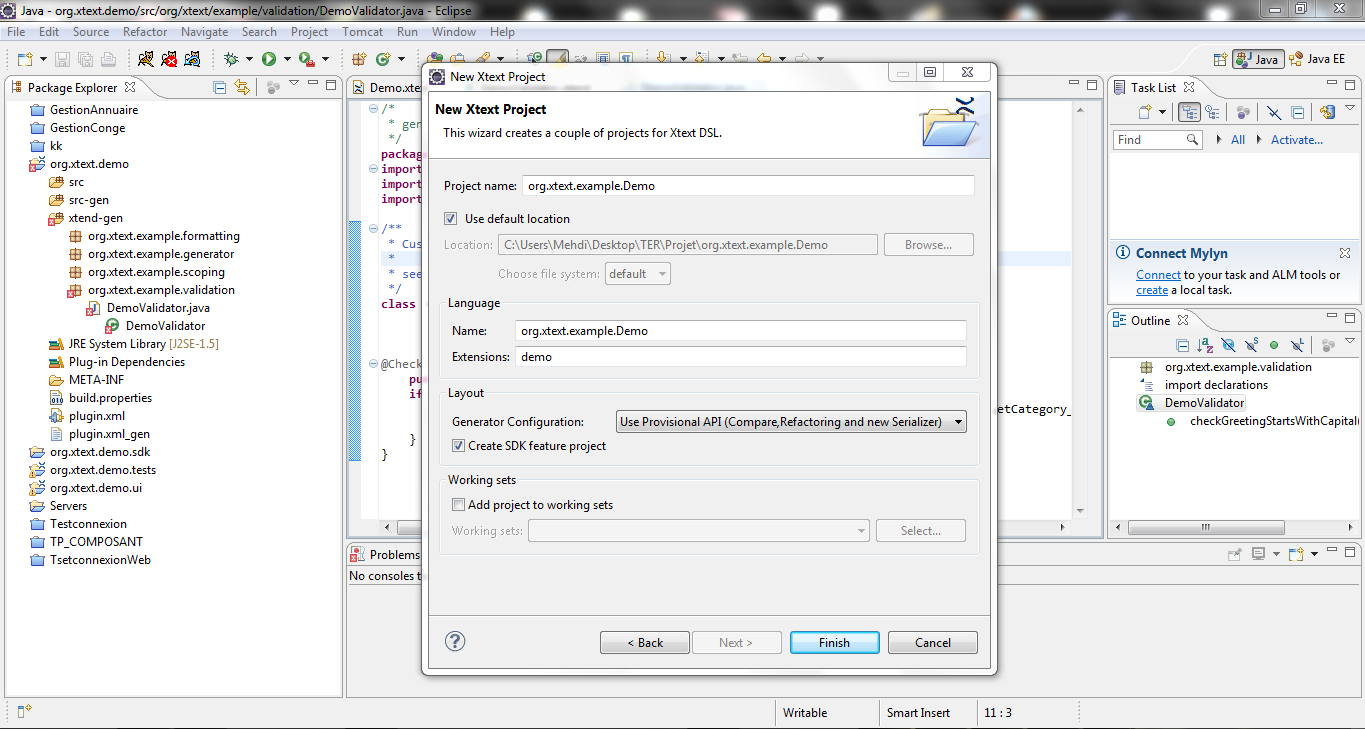
\includegraphics[width=1.10\textwidth,height=13cm]{1.PNG}
	\label{fig:1}
\end{figure}

Tout d'abord on va créer un projet Xtext avec comme nom et extension demo.A la fin de la creation, on remarque que EClipse à generer 3 projets, le premier c'est la ou on va definir notre langage, le deuxieme pour les tests et le troisieme ça concerne l'interface graphique de l'utilisateur.

\subsubsubsection{Etape 2:Definition du langage}


\begin{figure}[h]
	\centering
		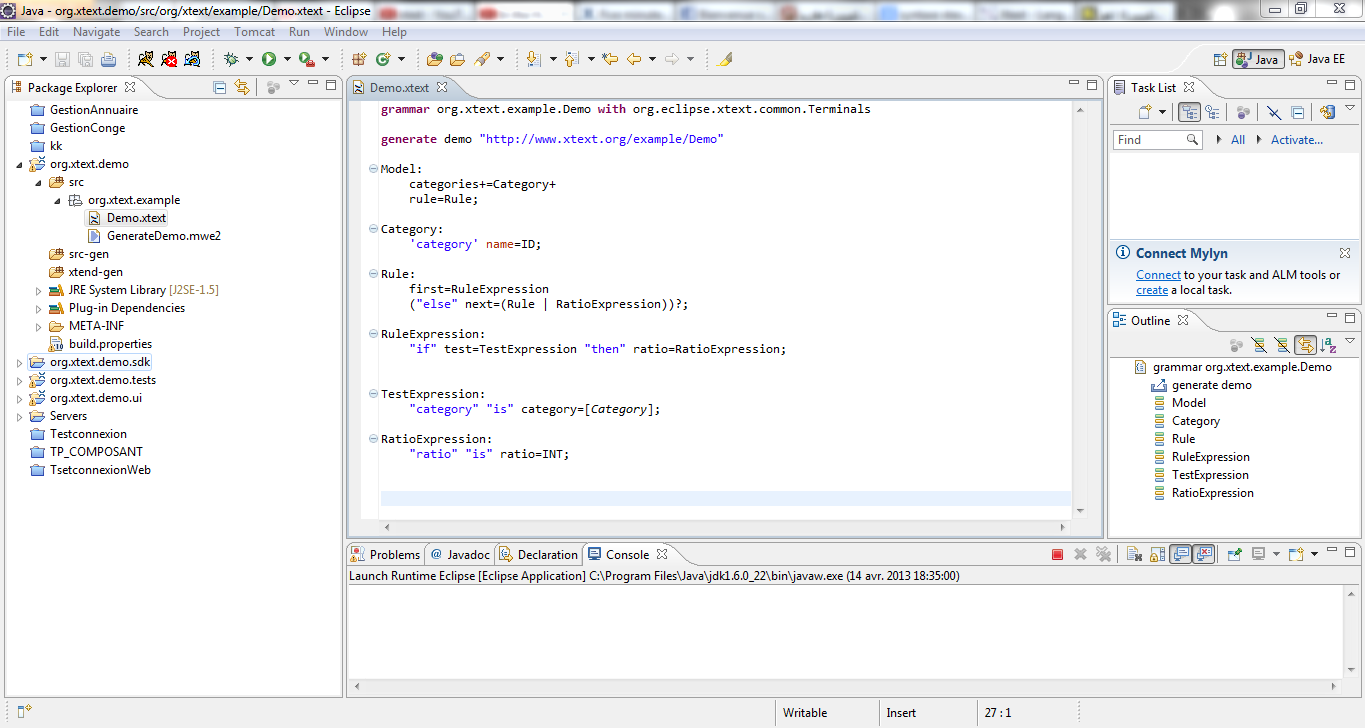
\includegraphics[width=1.10\textwidth,height=13cm]{2.PNG}
	\label{fig:2}
\end{figure}




\newpage









\section{Conclusion}
\label{hints}

\section{Références}
\label{hints}
\section{Some small hints}
\label{hints}
\subsection{German Umlauts and other Language Specific Characters}
\label{umlauts}
You can type german umlauts like 'ä', 'ö', or 'ü' directly in this file.
This is also true for other language specific characters like 'é', 'è' etc.
There are problems with automatic hyphenation when using language
specific characters and OT1-encoded fonts. In this case, use a
T1-encoded Type1-font like the Latin Modern font family (\verb#\usepackage{lmodern}#).
\subsection{References}
\label{references}
Using the commands \verb#\label{name}# and \verb#\ref{name}# you are able
to use references in your document. Advantage: You do not need to think
about numerations, because \LaTeX\ is doing that for you.
For example, in section \ref{dividing} on page \pageref{dividing} hints for
dividing large documents are given.
Certainly, references do also work for tables, figures, formulas\ldots
Please notice, that \LaTeX\ usually needs more than one run (mostly 2) to
resolve those references correctly.
\subsection{Dividing Large Documents}
\label{dividing}
You can divide your \LaTeX-Document into an arbitrary number of \TeX-Files
to avoid too big and therefore unhandy files (e.g. one file for every chapter).
For this, you insert in your main file (this one) for every subfile
the command '\verb#\input{subfile}#'. This leads to the same behavior
as if the content of the subfile would be at the place of the
\verb#\input#-Command.


\appendix
%-----------------------------------------------------------
\section{Introduction}\label{sec:intro}

Prérequis:
\begin{itemize}
\item Un fichier \texttt{*.tex}, par exemple \texttt{rapport.tex}, qui
  contient le texte.
\item Un fichier \texttt{*.bib}, par exemple \texttt{rapport.bib}, qui
  contient les références bibliographiques.
\end{itemize}

Utilisation de Latex:
\begin{itemize}
\item Lancer \texttt{pdflatex rapport} pour compilation du fichier
  \texttt{rapport.tex}
\item Lancer \texttt{biblatex rapport} pour compilation du fichier
  \texttt{rapport.bib}
\item Répéter \texttt{pdflatex rapport} deux fois pour prendre en
  compte des modifications
\end{itemize}

Documentation:
\begin{itemize}
\item \LaTeX: \url{http://www.latex-project.org/}
\item \TeX users group: \url{http://www.tug.org/}
\end{itemize}


%-----------------------------------------------------------
\section{Présentation du projet}

\subsection{But du projet}
On a utilisé
\cite{lindholm99_java_virtual_machin_specif,moore89_system_verif} et
aussi \cite{strecker02_verif_java_compil}.

\subsection{Implantation}

\begin{figure}[htbp]
  \centering
% \includegraphics[scale=0.5]{foo}
  \caption{Une petite image}
  \label{fig:im}
\end{figure}

Inclusion d'images en format PDF (création par exemple avec
XFig\footnote{Page web: \url{http://www.xfig.org/}})

\subsection{Spécialités}

Facile à utiliser: Listes d'éléments numérotés:
\begin{enumerate}
\item premier élément
\item deuxième élément
\item aussi imbriqués:
%
\begin{itemize}
\item Ici, une liste non numérotée
\item avec un autre élément
\end{itemize}
%
\end{enumerate}

Mathématiques:
\begin{itemize}
\item Sous- et super-scripts: $a_n$ et $b^k$, utiliser des accolades
  pour des expressions plus complexes: $x^{(y^z)}$

\item Symboles mathématiques, tels que $\sum_{i=0}^{n} f(i)$

\item Caractères de l'alphabet grecque: $\Gamma$ ou calligraphiques: ${\cal D}$
\end{itemize}

Fontes de caractères spécifiques:
\begin{itemize}
\item \emph{Italique}
\item \textbf{Gras}
\item \texttt{typewriter}
\item ou combiné \emph{\textbf{italique-gras}}
\end{itemize}

%-----------------------------------------------------------
\section{Gestion du projet}

\begin{tabular}[h]{|l|l|}
\hline
Dates & Tâches \\
\hline
\hline
Du 7 mars au 2 mai & 1~ière itération \\
                   & 2~ième itération \\
\hline
\end{tabular}

Je me réfère à la section~\ref{sec:intro} et la figure~\ref{fig:im}.

%-----------------------------------------------------------
\bibliography{bibliographie}
\bibliographystyle{abbrv}
\end{document}

%%% Local Variables:
%%% mode: latex
%%% TeX-master: t
%%% coding: utf-8
%%% End:
